\documentclass{article}

%%%%%%%%%%%%%%%%%%%%%%%%%
%%% Packages %%%%%%%%%%%%
%%%%%%%%%%%%%%%%%%%%%%%%%

% UTF8 characters
\usepackage[utf8]{inputenc}
\usepackage[english]{babel}

% Paper size
\usepackage[a4paper, total={6in, 8in}]{geometry}

% include pdfs
\usepackage{pdfpages}

% this loads a comment environment
\usepackage{verbatim}

% space between paragraphs
\usepackage{parskip}

% create listings for code examples
\usepackage{listings}

% inset time automatically
\usepackage[nodayofweek]{datetime}

% load additional colors
\usepackage{xcolor}

% count within figures (used in appendix for figures)
\usepackage{chngcntr}

% include graphics
\usepackage{graphicx}

% underline text
\usepackage{ulem}

% math stuff
\usepackage{amsmath,amssymb}

\usepackage[utf8]{inputenc}

% place figures and listings where they belong
\usepackage{float}
\floatplacement{figure}{H}
\floatplacement{lstinputlisting}{H}

\setlength{\arrayrulewidth}{1mm}
\setlength{\tabcolsep}{18pt}
\renewcommand{\arraystretch}{1.5}

\usepackage{adjustbox}

\begin{document}

\section{Analyzer}

\textbf {Can you explain the performance differences between the different versions using some
analysis tool, e.g. analyzer? Does the tool confirm your expectations}?

\begin{figure}[H]
  \centering
  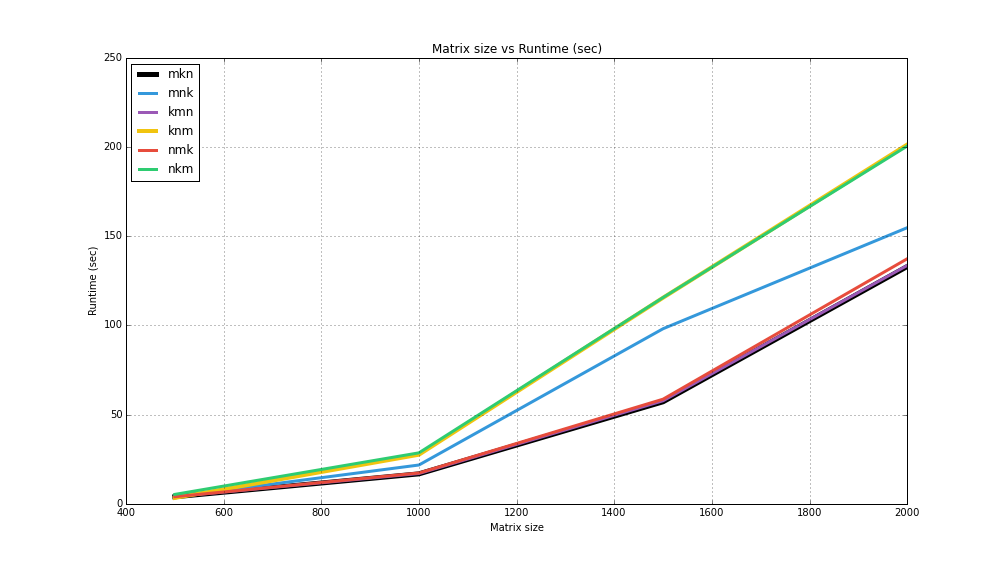
\includegraphics[scale=0.5]{Runtime.png}
  \caption{Plot for the six different permutations, matrix sizes vs. runtime, square matrices of 500, 1000, 1500 and 2000.}
 \label{fig:plot_runtime}
\end{figure}

\begin{adjustbox}{max width=\textwidth,center}
	\begin{center}
    \begin{tabular}{| l | l | l | l | l |}
    \hline
    Permutations & m=n=k=500 & m=n=k=1000 & m=n=k=1500 & m=n=k=2000  \\ \hline
    mkn & 4.050 s & 16.880 s & 57.250 s & 132.990 s \\ \hline
    kmn & 4.110 s & 17.070 s & 57.820 s & 133.580 s \\ \hline
    nmk & 4.080 s & 17.370 s & 58.710 s & 137.330 s \\ \hline
    mnk & 4.080 s & 21.840 s & 98.160 s & 154.730 s \\ \hline
    nkm & 5.380 s & 28.650 s & 115.640 s & 200.460 s \\ \hline
    knm & 3.410 s & 27.610 s & 115.520 s & 201.300 s \\ \hline
    \end{tabular}
\end{center}
\end{adjustbox}

\begin{figure}[H]
  \centering
  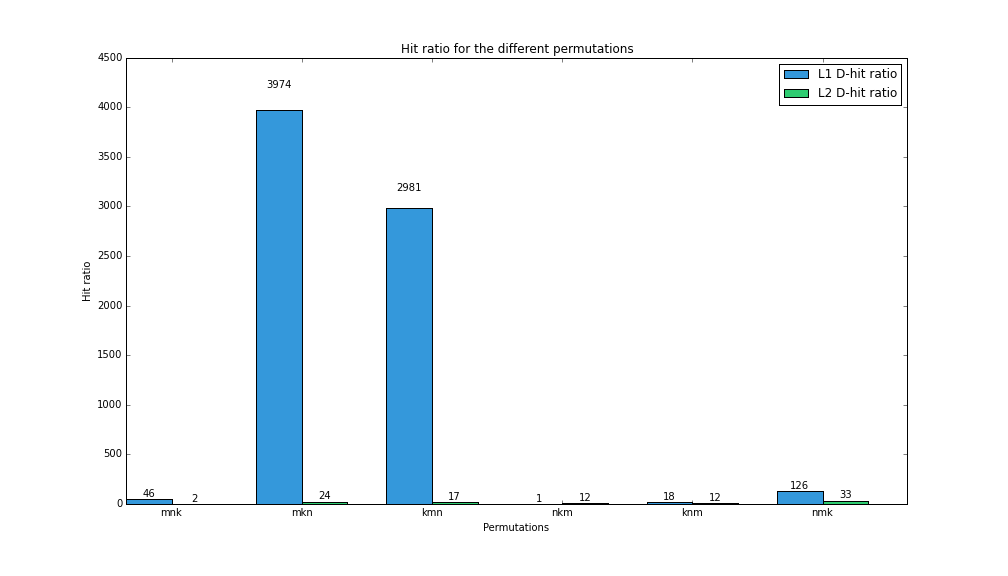
\includegraphics[scale=0.5]{hitratio.png}
  \caption{Plot for hit ratio vs. permutations, square matrix of 500, mflops\_max\_it of 50.}
 \label{fig:plot_hit ratio}
\end{figure}

\[ Cache Refs - Cache Misses / Cache Misses = Hit Ratio \]

\begin{adjustbox}{max width=\textwidth,center}
	\begin{center}
    \begin{tabular}{| l | l | l | l | l | l | l  |}
    \hline
    L2 D & mnk & mkn & kmn & nkm & knm & nmk  \\ \hline
    Cache Refs & 100815940823 & 150726065855 & 150738548844 & 15124047909 &
151263541727 & 150757006506 \\ \hline
    Cache Misses & 2169988937 & 37921061 & 
50562333 & 8271302759 & 8254503877 & 1192497865 \\ \hline
    Hit Ratio & 46.4591 & 3974.7322 & 2981.2419 & 1.8284	& 18.3249 & 126.4211 \\
    \hline
    \end{tabular}
\end{center}
\end{adjustbox}


\begin{adjustbox}{max width=\textwidth,center}
\begin{center}
    \begin{tabular}{| l | l | l | l | l | l | l  |}
    \hline
    L1 D & mnk & mkn & kmn & nkm & knm & nmk  \\ \hline
    Cache Refs & 2337185157 & 808373113 & 816761066 & 9726740774 &
9827651083 & 2025085625 \\ \hline
    Cache Misses & 790190116 & 33302649 & 
46629262 & 808869156 & 794451254 & 59968558 \\ \hline
    Hit Ratio & 2.9597 & 24.27 & 17.516 & 12.025	& 12.3703 & 33.7691 \\
    \hline
    \end{tabular}
\end{center}
\end{adjustbox}

A cache miss, generally, is when something is looked up in the cache and is not found. The cache did not contain the item being looked up. The cache hit is when you look something up in a cache and it was storing the item and is able to satisfy the query.

We saw previously that "mkn" has the lowest runtime followed by "kmn". Therefore, they should have the highest hit ratio. We can clearly see in figure 2 that the expectation is confirmed. The faster the algorithm runs the higher hit ratio it has. This makes sense. In order to have a high hit ratio, there are many hits and few misses. If there are many hits the data is stored in the local memory cache. Therefore, the thread runs fast.

The slower the algorithm runs the lower is the hit ratio. This is understandable as well. In order to have a low hit ratio, there are few hits and many misses. If there are many misses, this means the data is not stored in the local memory cache. The hardware has to then make a number of requests to main memory to fill up the local memory cache which causes the thread to run slower.

\end{document}